\chapter{METHODOLOGY AND RESULTS}

\sepfootnotecontent{fn:unity-engine}{[Footnote: What is the Unity engine]}

\sepfootnotecontent{fn:triple-a}{AAA (pronounced "triple A") games are an informal classification of video games distributed by major publishers and distinguished by large development and marketing budgets. In general, the term is used to represent the games that are supposed to achieve the highest standard of quality and content in video games.}

\sepfootnotecontent{fn:genshin-impact}{Genshin Impact (miHoYo, 2020). Video Game. Android, iOS, Windows, PlayStation 4, Playstation 5, Nintendo Switch.}

\sepfootnotecontent{fn:escape-tarkov}{Escape from Tarkov (Battlestate Games, 2017). Computer Game. Microsoft Windows.}

\sepfootnotecontent{fn:hollow-knight}{Hollow Knight (Team Cherry, 2017). Video Game. PlayStation 4, Nintendo Switch, Xbox One, macOS, Linux, Microsoft Windows.}

\sepfootnotecontent{fn:ghost-tale}{Ghost of a Tale (SeithCG \& Plug In Digital, 2016). Video Game. PlayStation 4, Nintendo Switch, Microsoft Windows, Xbox One.}

\sepfootnotecontent{fn:cuphead}{Cuphead (Studio MDHR Entertainment Inc., 2017). Video Game. PlayStation 4, Nintendo Switch, Xbox One, Microsoft Windows, macOS.}

\sepfootnotecontent{fn:undead}{\emph{Undead} beings are fictional characters represented by entities that were reanimated from death through supernatural means. Common representations of \emph{Undead} beings in popular media include \emph{Zombies}, \emph{Skeletons} and \emph{Vampires}.}

\sepfootnotecontent{fn:particle-vfx}{Footnote: What are particle-based visual effects}

\sepfootnotecontent{fn:death-stranding}{Footnote: What is Death Stranding}

\sepfootnotecontent{fn:core-gameplay-loop}{Footnote: What is the Core Gameplay Loop}

\sepfootnotecontent{fn:character-controller}{Footnote: What are CharacterControllers}

\sepfootnotecontent{fn:movement-drifting}{Footnote: What is movement drifting}

\sepfootnotecontent{fn:lock-on}{Footnote: What is Lock-On targeting}

\sepfootnotecontent{fn:colliders}{Footnote: What is a collider}

\sepfootnotecontent{fn:collider-overlapping}{Footnote: What is collider overlapping}

\sepfootnotecontent{fn:monobehaviour}{Footnote: What is a MonoBehaviour}

\sepfootnotecontent{fn:fixed-update}{Footnote: What is the FixedUpdate timestep}

\sepfootnotecontent{fn:rays}{Footnote: What are rays}

\sepfootnotecontent{fn:raycasts}{Footnote: What are Raycasts}

\sepfootnotecontent{fn:mecanim}{Footnote: What is the Mecanim system}

\sepfootnotecontent{fn:skeletal-rigs}{Footnote: What are skeletal rigs}

\sepfootnotecontent{fn:motion-sickness}{Footnote: What is motion sickness}

\sepfootnotecontent{fn:unity-prefabs}{Footnote: What are Unity Prefabs}

\sepfootnotecontent{fn:unity-gameobjects}{Footnote: What are Unity GameObjects}

\sepfootnotecontent{fn:transposing-and-composing}{Footnote: What are Transposing and Composing strategies}

\sepfootnotecontent{fn:observer-pattern}{Footnote: What is the Observer pattern}

% ============================================================================
% ============================================================================
% ============================================================================

\section{Overview}

% About the analysis of Dark Souls

% About our implementation of Dark Souls "Core"

% About our implementation of DDA

% About the process of our Experiment

% About the results comparing to previous DDA Systems

% ============================================================================
% ============================================================================
% ============================================================================

\section{Analysis of Dark Souls}
\label{sec:analysis-dark-souls}

In this section, we analyze the Game Design of our object of study to define the essential aspects required to implement a replica of its core elements and experience. We argue that understanding the Game Design of \emph{Dark Souls} is crucial to the interpretation of difficulty in games. While \emph{Dark Souls} presents a wide variety of mechanics and interactions, only the basic rules required for the implementation of the combat system will be described.

% ============================================================================
% ============================================================================
% ============================================================================

\subsection{Motivation of Choice}

Dark Souls has successfully pushed the extents of challenge in Action RPGs to their limit, providing combat with a simple yet carefully designed set of core mechanics. However, the greatest capability of the \emph{Dark Souls} series, the design of its difficulty, is for some an unwelcome trait. While having enemies with simple pattern-based AI, the game punishes players heavily for making the slightest mistakes. For this reason, \emph{Dark Souls} is often mentioned as a reference to difficulty in games \cite{URL_ExploringDesignOfDarkSouls}.

The player does not fail in \emph{Dark Souls} by dying, but by giving up on finishing the game. The game design creates a cycle of experimenting, dying, learning, adapting and only then progressing through the levels. Therefore death is not considered failure, but simply the price paid for knowledge. Because of this type of punishing yet rewarding design, the special edition of the first title in the \emph{Dark Souls} series yields the subtitle "Prepare to Die Edition".

While the average action game might reward the player for beating entire armies of enemies on his own, \emph{Dark Souls} can be a rewarding experience for the player even when basic encounters are surpassed, such as surviving a battle with a single enemy. When adventuring through the tight corridors of a dungeon or dark underground caves, the player faces unknown dangers and must fight their way out. Even the weakest enemies can surprise and kill an unsuspecting player. When facing the strong opponents, dealing the finishing blow in an intense fight means the player overcame a challenge.

Understanding the design of Dark Souls is, therefore, a key component to understanding the relationship of challenge and reward.

% ============================================================================
% ============================================================================
% ============================================================================

\subsection{Overview of Aesthetics}

% ============================================================================
% ============================================================================
% ============================================================================

\subsection{Overview of Game Mechanics}

\emph{Dark Souls} is for the most part presented in a Third Person Camera perspective, with the player character positioned close to the center of the screen. The Third Person perspective is distinguished by the visibility of the player character's model and actions and a slight view of their surroundings.

In comparison to First Person Camera Systems, and considering only mechanical gameplay aspects, Third Person Cameras are better suited to action games with platforming sections. In these sections, the player must have full control and awareness over the character position to avoid falling to their death. Third person perspectives also succeed in close-combat games by providing a broad view when the player deals with multiple enemies simultaneously.

However, as seen in \cite{BOOK_LevelUpTheGuideToGreat}, Third Person Cameras often have a problem of visibility in regards to the player character in tight or confined spaces of the game world, such as corridors and small rooms. The camera must be confined inside the game level boundaries to prevent inappropriate viewing of elements of the environment, such as  out-of-bounds artifacts.

In a Orbital Third Person Camera System, character movement is based upon the relationship of character position to the camera orientation \cite{BOOK_RealTimeCameras}. If the player moves forward, the character moves towards the direction the camera is facing. In Dark Souls, moving sideways also causes the camera to slightly rotate towards the direction of the movement. Therefore, if the player constantly moves horizontally without adjusting the camera, the character will move in a circle.

In situations where the camera position is invalid, the camera should reposition inside the playable bounds of the environment whenever the intended default position of the camera would be out of the limits or inside an object. According to \cite{BOOK_RealTimeCameras}, there is no standard solution to this issue. In Dark Souls, the adopted solution is to simply pull the camera closer to the player character. The relative size of the player in screen is then greatly increased and might disrupt the visualization of important gameplay elements. 

Environment elements such as columns, rocks or even non-playable characters might impair the visualization of the player character and non-player characters, thus hindering the combat capabilities of the player. In response, Third Person games with close-quarters combat often present the "Lock-On" camera as an alternative to the default.

A View Locking Camera System, such as the Lock-On Camera, overrides the orientation of a Third Person Camera by locking the orientation of the view to a "lock target". Instead of centering on the player character, the Lock-On Camera focuses on another object or position such as a non-playable character, while still offsetting the position of the player character. This allows the visualization of the two essential elements in a combat encounter: the player character and their enemy.

In the View Locking Camera System, the player movement method changes to a circular strafe relative to the lock target position. Moving sideways results in an arc-shaped motion around the target. Forward and backwards movement transposes the player character closer to or away from the target.

The Lock-On Camera is ideal for single-target combat situations, as the player can avoid enemy attacks sideways while still keeping a desirable distance to counterattack. Area of Effect attacks which affect any entity in a circular area around the enemy can also be easily avoided by moving away from the enemy. In the case of Dark Souls, the player character orientation is updated to constantly face the target, thus simplifying the process of directing attacks at enemies. Since the player character is constantly facing the direction of the target, successfully registering the attack simply requires the player to position their character in range of the target.

Dark Souls is an Action RPG with heavy focus on close-quarters combat. In contrast to other games in the genre, the combat does not present itself as fast-paced or dynamic. Instead, the game focuses on realism and slow but strategic movements. According to \cite{BOOK_DarkSoulsBeyondTheGrave}, \emph{Dark Souls} respects its predecessors such as \emph{King's Field} with a feeling of weight and impact on hits, emphasizing the necessity of players to protect themselves behind a shield.

The controls in any game of the \emph{Souls} series operate in similar fashion: each of the character's arms are controlled by separate buttons, represented by the left and right shoulder pad in a Joystick. The player can wield different one-handed equipments in each arm, or a two-handed equipment in both arms. The character will perform actions for an arm based on which equipment is equipped, such as slashing with a sword or defending with a shield. If a two-handed weapon is equipped, using the right shoulder pad button will attack and the left will defend. The most common configuration is to have a shield in the left hand, and a weapon in the right.

During play-through, the player will come across a wide variety of weapons with different attacks, but the same core functionality. Each attack requires a certain amount of \emph{Stamina}, deals a certain amount of \emph{Damage} and has a \emph{Recover Time} after the action. Certain attacks also have the chance of \emph{Staggering} an enemy. These core concepts are strategic factors the player must consider before taking action. 

\begin{itemize}

\item \emph{Damage}: the amount of health a character loses upon getting struck by an attack. This amount can be reduced or fully negated by blocking or dodging incoming attacks.

\item \emph{Health}: an attribute representing the overall physical state of a character. Numerically, it determines how much Damage a character can sustain before being destroyed.

\item \emph{Stamina}: an attribute that represents the character tiredness. Numerically, it determines the ability to perform actions in combat. Attacking, dodging and even shielding oneself against enemy attacks all have a \emph{Stamina} cost. Although \emph{Stamina} is a finite resource, it replenishes passively after the player stops performing combat actions.

\item \emph{Recover Time}: the amount of frames the player is unable to do any actions and is vulnerable to attacks after their own attack has taken place. This attribute is used to create a feeling of weight in attacks, and can be used by the player to punish slow enemies after missing an attack.

\item \emph{Stagger}: the condition where a character is unable to perform any actions and is vulnerable to attacks after getting struck by a powerful attack or a quick succession of attacks. In \emph{Dark Souls}, this condition is especially cruel to the player, since after losing a significant amount of health the player is still susceptible to a follow-up attacks, without the ability to defend their self.

\end{itemize}

In general, Heavy attacks are slower and cost the most Stamina, but deal the highest damage and \emph{Stagger} the enemy. Light attacks are faster and can be linked for a quick succession of attacks, but deal individually less damage while having a low chance of causing \emph{Stagger}.

As means of defense, a player can Block, Dodge, Parry or simply move away from an attack. Blocking requires the player to have their shield lifted at the time of the attack. Each block costs an amount of Stamina based on the power of the attack and the character's resistances. If an enemy attack is too powerful and the character does not have the required Stamina, they may still enter a Stagger condition. Out of all the defensive actions, Blocking is the safest and least skill dependent, since it will only fail if the attack hits the back of a character. While blocking, the player will replenish Stamina at a reduced rate.

Dodging can be performed by rolling in the right direction with precise timing. While costing Stamina, succeeding in this action completely negates the damage of an attack, ignoring how powerful it is. Upon failing, the character will take full damage. Thus, this action should be performed with care and heavily depends on the player reflexes.

Similarly to Dodging, Parrying can be performed with precise timing to deflect an enemy attack and destabilize the enemy. The player can then perform a riposte attack, a powerful move that adds a considerable amount of damage. Failing a Parry will cause the player to take full damage of the attack. Parrying is harder than dodging, since time window to perform the action is considerably smaller. Thus, Parrying is a high-risk high-reward action, and can also be considered an offensive move.

However, Blocking, Parrying and Dodging require the usage of Stamina, a valuable resource which is also required to perform offensive moves. If a player only blocks incoming attacks, their Stamina will not replenish quickly enough to sustain attacks indefinitely. Moreover, if a player faces multiple enemies, blocking can sustain even less attacks, and quickly deplete the player Stamina. Dodging and Parrying are timing dependent, and thus prone to mistakes and heavy punishment. If players repeatedly try to perform the same defensive action, they will often find themselves cornered, without Stamina and vulnerable to fatal blows. Experienced players have the knowledge of when they should perform none of these actions, instead simple moving away and creating space for favorable counterattack opportunities.

% ============================================================================
% ============================================================================
% ============================================================================

\subsection{Artificial Intelligence}

Upon the research conducted in the creation of this work, no official information on the implementation of the AI in Dark Souls was discovered. According to \citeonline{YT_DarkSoulsSimpleAI}, some sources indicate a \emph{Hierarchical Task Planning Network System}, but an analysis of the in-game enemy actions provides no support to this claim. However, by multiple tests and playthroughs, it was possible to reverse engineer the behavior of enemies and suggest a replication formulae in the implementation of this work.

Non-player characters often share similar behavioral patterns in Dark Souls. Whi\hyp{}le the actions of a humanoid NPC might differ from a quadruped, their overall behavior upon player presence is the same. The NPC stands idle until receiving interaction from their sensors, such as the player stepping into their line of sight. At that point, the enemy will either attack at range, if using a bow or spell, or rush towards the player and attack in close-quarters.

Enemies wearing a shield will commonly attempt to defend themselves when the player repeatedly attacks. The defense stance can be punished by the player when they perform a kick or by attacking from behind. In other occasions, a low health enemy might evade attacks or even heal itself. Most of these strategies are predictable, even when there is a variability in the patterns used.

Ultimately, the AI of Dark Souls is simplistic, but sufficient for the objectives proposed by the developer. The predictability of this system can be considered a favorable factor for a player learning how to overcome an enemy. This simplicity is not perceivable by the player in the first playthrough, since the player will struggle with the challenging aspects of the level design. In addition, Dark Souls present its enemies as being overtly strong in comparison to the player. A slight mistake might cause the player to endure punishing amounts of damage, thus creating the illusion of a difficult opponent.

The perception of strength in Dark Souls's enemies carries similarities to the development of the original \emph{Halo} by Bungie. According to \citeonline{URL_IllusionOfIntelligence}, players perceived the smartness of an enemy based on their endurance and damage dealt to the player. Simply increasing the Health points of an enemy enhanced the first perception of enemies intelligence for playtesters. This perception of toughness could shadow the lack of intelligence of an enemy in a first playthrough. However, as the player repeatedly faces the same enemy upon countless deaths, this illusion is gradually faded.

% ============================================================================
% ============================================================================
% ============================================================================

\subsection{Level Design}

According to \cite{BOOK_LevelDesignConcept}, Level Design can be defined as an interpretation of Game Design. The Level Designer must understand the rules of a game and determine how a player is confronted by them. It can be argued that Game Design represents the theoretical part of a game, whereas Level Design applies it in practice.

Level Design determines the layout of a location, the placement of enemies, the gameplay objects and the environmental hazards. In a sense, Level Design can be seen as a means of expressing Game Design through an exploration narrative. Therefore, a game developer must consider what experiences the player is supposed to face in a section before tackling on its design.

In the case of Dark Souls, the world takes place in an open, interconnected and vertically stacked map layout. When projecting this layout on a two-dimensional chart, it resembles the format of a spiral. This type of map layout is radically different than other games in the genre such as \emph{The Elder Scrolls V: Skyrim} \footnote{The Elder Scrolls V: Skyrim (Bethesda Game Studios, 2011). Computer Game. Microsoft Windows.}, which presents  dungeon maps as horizontally spaced and linear paths.

By journeying through the world, the player will come across castles, dungeons, caves, and fortresses. It is more frequent to find oneself in small passageways than open areas, the latter being used more often in \emph{boss fights}. The need of constantly turning left and right, ascending stairs and descending through dark passages gives the developers numerous places to hide enemies and traps in. Thus, the player often faces threats such as being assaulted by an unseen enemy, getting hit by a trap or even falling to their death.

Each and every enemy the player faces has the potential to generate a difficult encounter. An enemy that is considered weak can still take away a considerable amount of Health from the player. However, enemies are commonly vulnerable after performing an attack, and thus open for an instant kill. Therefore, the player has the possibility of optimizing their play style by spotting enemies ahead of time, planning on how to exploit weaknesses and only then performing the action.

The strength of a \emph{Souls}-like game isn't just its combat. When every little bit of a level can be threatening, it encourages the player to experience the atmosphere and story of the world. The careful placement of enemies, traps and pitfalls in creative fashion constitutes the core of \emph{Dark Souls} Level Design.

A Dark Souls player is encouraged to memorize whole map sections to progress withstanding minimal damage. The constant feeling of danger increases the tension and maintains the player aware of their situation to survive. According to \citeonline{YT_EvolutionOfDarkSoulsLevelDesign}, the Level Design in  Dark Souls is the main contributor to the player immersion in the game's narrative.

However, the pitfalls and traps of Dark Souls can be spotted ahead of time if the player decides to maintain a slow pacing an pay attention to their surroundings. This characteristic makes the seemingly unfair encounters beatable. Groups can be separated into smaller sizes by luring enemies one by one. The environment traps can be used against the enemies, if the player lures the target to the area of effect. Enemies can be pulled from their territory into a safer and player-controlled position.

Spiral level designs can also feature alternate routes and shortcuts. Since the player is constantly facing the danger of losing Experience Points upon dying, the Spiral layout provides the player with shorter paths and less risk when returning to safe zones. In the same philosophy, the game will often contain shortcuts from safe zones to later attained areas. These shortcuts must be unlocked by reaching a certain location and performing an action, such as finding the key to a locked gate. This Level Design technique is commonly known as \emph{gating} \cite{BOOK_LevelUpTheGuideToGreat}.

% ============================================================================
% ============================================================================
% ============================================================================

\subsection{The "Pain Points" of Dark Souls for Beginner-Level Players}

% ============================================================================
% ============================================================================
% ============================================================================

\section{System Architecture, Design and Implementation}

% Brief description of all subsections: Tools and Frameworks, Game Assets and Aesthetics, Gameplay Mechanics and Systems, Artificial Intelligence, Telemetry and Performance Tracking, Dynamic Adjustments
In this section, we specify the details for each of the major decisions and systems for the implementation of an appropriate replica of the core elements of Dark souls with the additional aspect of an adaptive system that dynamically adjusts game difficulty to the profile of a player. We provide a detailed list of the requirements of our implementation, along with the motivation for the choice of each technology and game asset.

We specify the design and implementation of the gameplay mechanics and systems in Bright Souls, using a restricted set of the elements in the original game as a reference and comparing it to our previous analysis from section \ref{sec:analysis-dark-souls}.

% ============================================================================
% ============================================================================
% ============================================================================

\subsection{Tools and Frameworks}

% Brief overview of tools used in the project, specify that we chose Unity, Cinemachine, Post Processing Stack, Aura Volumetric Rendering

In order to implement an appropriate replica of the main elements that compose Dark Souls, we first require a framework that can provide the tools to assemble and render 3D environments with high visual fidelity. Then, it is useful to have a set of utilities and ready-to-use systems to implement the functional aspects of the original game, such as a standardized Input System that can deal with multiple input devices, a set of definitions and functions to manipulate 3D Camera behavior and control and a physics engine that can detect and handle collisions for at least basic geometry such as bounding boxes. For these reasons, we chose \emph{Unity}\sepfootnote{fn:unity-engine} as our development platform as it contains most of the essential functionality we require, with the added possibility of extending and adapting the purpose of its editor to satisfy any additional needs.

% Motivation for using Unity3D
% - A complete framework that is widely used in the industry, and is able to achieve AAA quality products with current examples in the industry;

Unity is widely used in the video games industry, with a feature-rich framework that supplies game developers with tools to achieve AAA\sepfootnote{fn:triple-a} quality products. Some examples of successful games implemented under Unity include Genshin Impact\sepfootnote{fn:genshin-impact}, Escape from Tarkov\sepfootnote{fn:escape-tarkov}, Hollow Knight\sepfootnote{fn:hollow-knight}, Ghost of a Tale\sepfootnote{fn:ghost-tale} and Cuphead\sepfootnote{fn:cuphead}.

% - A concise integrated editor that can be used for map editor, project folder organization, game data management;
Unity offers a concise, integrated project editor that offers functionality such as level editing, files and folders structural organization, game data management, in-game and serialized component inspection, a visual editor for serialized animation state machines, configuration options for deploying platforms and architectures, a debug console and tools for generating offline light mapping data for scene rendering.

% - A general API that provides the tools to implement virtually any type of game;
Unity also defines a streamlined API so developers can implement their custom game code in \textsc{C\#}, providing access to reusable functionality libraries and systems such as the component-based \textsc{MonoBehaviour} API, the serialized data \textsc{ScriptableObject} API, the Input and UI systems and even the Editor package, which permits the developer to extend the built-in functionality of the Unity Editor to develop Quality of Life tools for improved creation workflows.

% - Possibility to deploy in multiple platforms (Windows, Linux, macOS) with minimal changes in source code;
It is also possible to deploy Unity projects to multiple platforms such as Windows, Linux, macOS, PlayStation, Nintendo Switch and Xbox with minimal changes in code, as Unity's standardized API and builtin \textsc{IL2CPP} compiler translates Intermediate Language code into automatically generated \textsc{C++} code, which is then compiled into a native binary for each target platform.

% - Possibility to import free and paid assets from the Unity Asset Store for 3D Models, Animations, Sounds, UI Elements, Shaders, Post-Processing Effects, Visual Effects;
However, one of the key factors behind the choice of Unity as a platform was the possibility of including free and paid assets from the \emph{Unity Asset Store}, a digital platform for the distribution and acquisition of game assets such as 3D Models, Animations, Sounds, 2D UI Elements, Shaders, Post-Processing Effects and Visual Effects. Without this, it would be impossible for the authors to develop a game that would be sufficient to even remotely resemble the qualities of a AAA game such as Dark Souls. By acquiring and importing high-quality game assets into the project, it was possible to focus on the design and development of game systems, while also having AAA quality assets as a resource to work with.

% - Possibility to import plug-and-play APIs and systems such as Cinematic Camera behavior controllers, Third person Movement Controllers and Universal Input Device Managers that can be easily integrated into the project and development workflow;
% - Possibility to import and integrate multiple development tools that are tailored to the specific needs of the product being developed, such as data serialization utilities, map editor utilities, telemetry and database management tools and visual effect creation tools;
As for the implementation and reuse of infrastructural development tools and game systems, the Unity development team has in recent years made relevant effort towards modularized, plug-and-play systems with the \emph{Packages} system. The Packages system defines a streamlined workflow for importing game assets, editor utilities and engine functionalities, where it is possible to individually import packages that are specific to the requirements of a Project. For the scope of this work, one relevant example would be the \textsc{Cinemachine} package, which contains functionality and tools for manipulating 3D cameras with sophisticated behaviors, real-time configurable properties based on lenses for real-world cameras, and pre-configured implementations of common functionality for cameras in video games.

% - Authors had previous familiarity with the engine from personal and professional experience;
The final deciding factor for the choice of Unity as a development platform was the previous personal and professional background of the authors with the engine, having implemented a wide variety of 2D and 3D Games, VR Serious Games and data visualization tools under Unity. The familiarity with the provided APIs, along with the knowledge of how to achieve a steady and concise workflow permitted the authors to plan a robust architecture and select the appropriate tools to implement the core features of Dark Souls with an acceptable quality in comparison to the original game.

% ============================================================================
% ============================================================================
% ============================================================================

\subsection{Game Assets and Aesthetics}

% 3D Models, animations and sound assets were selected based on trying to replicate the same general 'feel' of Dark Souls
The assets for the implementation contained within this work were elected with the objective to serve as resources to attempt to replicate the general aesthetics of Dark Souls. Therefore, as a basis criteria for the selection of used assets, we use the brief analysis in section \ref{sec:analysis-dark-souls} as a reference to explore options in the Unity Asset Store within the \emph{'Dark Fantasy'} thematic subcategory.

% Fantasy Dungeon
First, we require a set of 3D models to assemble a playable 3D environment that satisfy the aesthetics of the 'Dark Fantasy' genre. For this purpose, we elected the asset pack \emph{Fantasy Dungeon} -- a collection of 3D models with a 'Ruined Castle' theme. The overall aesthetics and theme of this aspect pack appropriately resemble the sense of 'abandonment' in the original game. When considering functionality aspects, this pack contains modular 3D objects and pieces that can be easily assembled into a playable environment. Furthermore, the asset pack also contains pre-assembled scenes with appropriate lighting and optimized meshes, which were adapted to fit the requirements of our implementation.

\begin{figure}
    \caption{A selection of screenshots from pre-assembled scenes using the 3D assets from the Fantasy Dungeon asset pack.}
    \begin{center}
        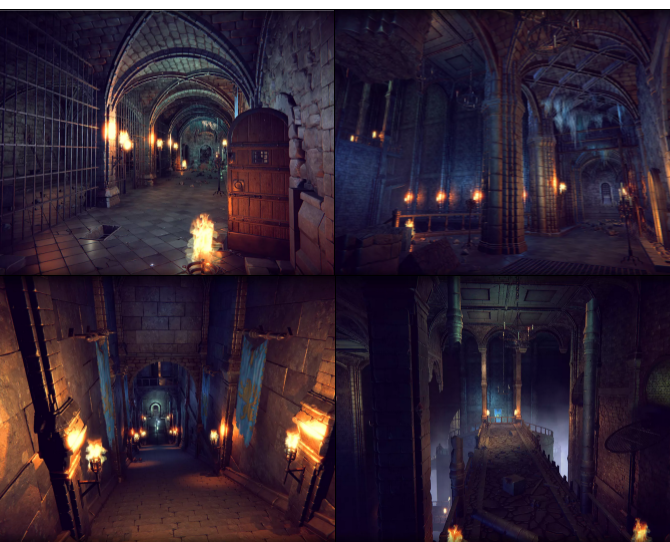
\includegraphics[width=24em]{figures/fig-environment-assets.png}
    \end{center}
    \legend{Source: Collation of screenshots performed by the authors from images captured from the original Unity Asset Store website pages for the \emph{Fantasy Dungeon} Unity asset.}
    \label{fig:environment-assets}
\end{figure}

% Then, we need 3D models for the Characters, The Blacksmith: Characters, Skeleton Zombies and Longsword Animset Pro

In sequence, we require 3D models to represent the playable character and any non-playable entities the player would be able to interact with. Regarding the non-playable entities, we attempt to implement enemy agents comparable to the enemies presented in the early levels of Dark Souls. Most of the enemies in these early sections of the original game are \emph{Undead}\sepfootnote{fn:undead} beings named \emph{'The Hollow'}, which are represented by creatures with decomposed skin and a dehydrated body that resemble the popular representation of \emph{Zombies}. In the original game, \emph{The Hollow} can be seen wearing a variety of attire, including ragged clothes, armored pieces such as cuirasses, pauldrons and helmets, bare skin or even without flesh in their bodies in the form of \emph{Skeletons}.

In addition to the requirement of being in harmony with the aesthetics of the original game, we also used as a criteria for the selection of enemy character models the requirement of serving a specific purpose in enemy behavior design and encounter design. Each enemy agent in our game should have a specific set of actions which can complement the actions of other enemies in a combat encounter. Therefore, we define enemy role archetypes based on the enemies seen in the initial levels of Dark Souls: the \emph{Ghoul}, the \emph{Archer}, the \emph{Swordsman} and the \emph{Assassin}.

Therefore, for the representation of enemy characters that satisfy our aesthetic and design requirements, we elected the asset packs \emph{Skeleton Zombies}, \emph{Longsword Animset Pro}, \emph{Modular Skeleton Archer}, \emph{Modular Skeleton Rogue} and \emph{Skeleton Humanoid}, all of which contain 3D models representing stereotypes of Zombies and Skeletons that resemble the enemies seen in the early stages of Dark Souls, while satisfying the roles we defined for the design of enemy agents in our implementation.

Another motivation for the selection of these asset packs was their compatibility with the \textsc{Mecanim}\sepfootnote{fn:mecanim} system, which standardizes \emph{skeletal rig}\sepfootnote{fn:skeletal-rigs} definitions for animations in humanoid characters in the \textsc{Unity} engine. When compatible with this system, character models can be used in combination with most animations that can be found in the \textsc{Unity Asset Store}, which provides the possibility of choosing from a wide collection of animation sets for multiple purposes, including animations for weapons wielded by the enemy characters we designed for our implementation.

\begin{figure}
    \caption{A mosaic portraying the 3D character models in Bright Souls.}
    \begin{center}
        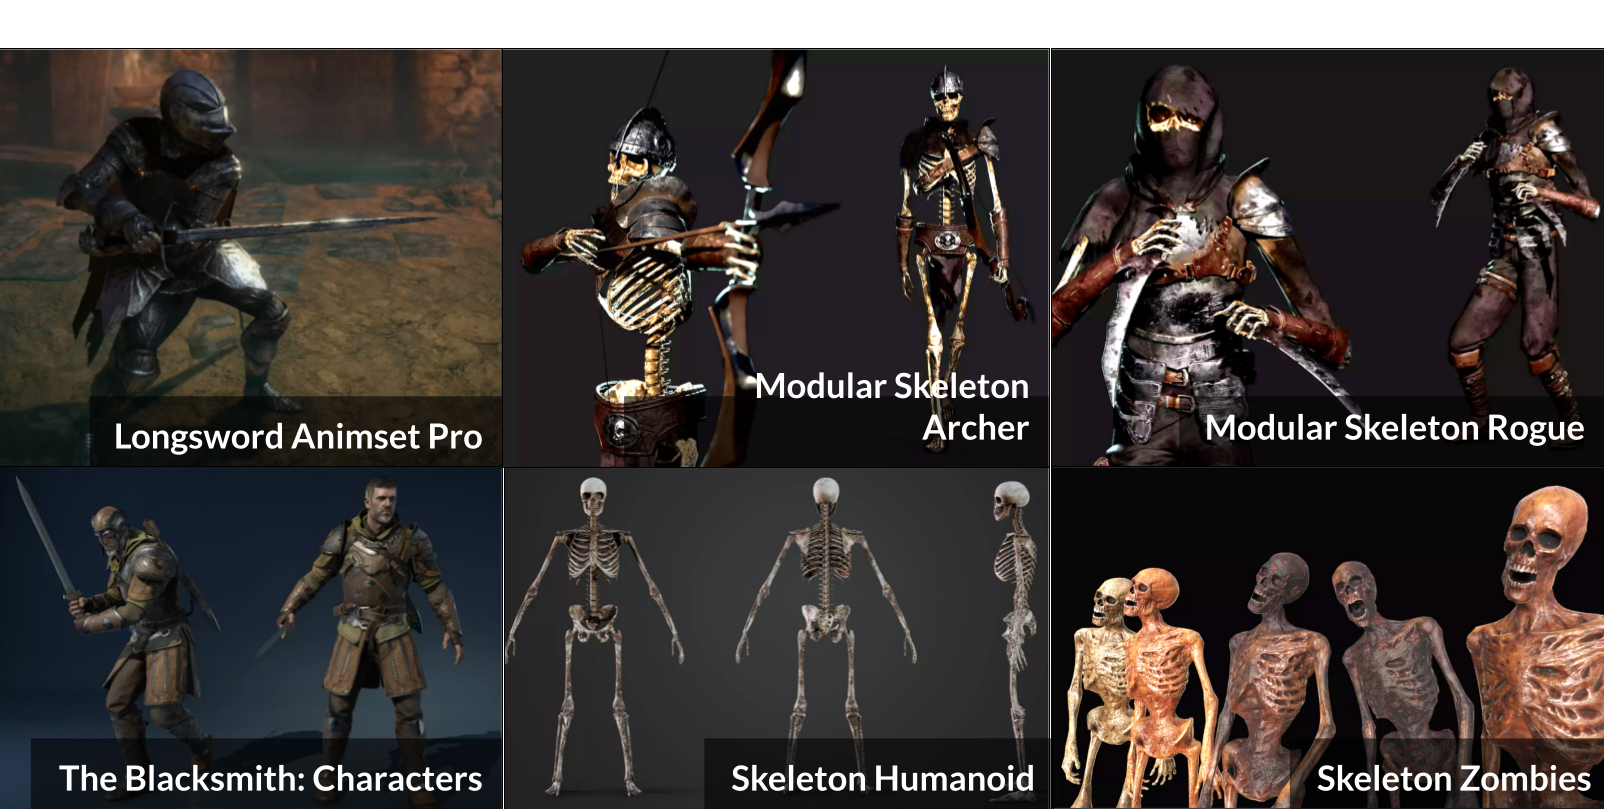
\includegraphics[width=30em]{figures/fig-character-assets.png}
    \end{center}
    \legend{Source: Collation of screenshots performed by the authors from images captured from the original Unity Asset Store website pages for each of the assets used in this work.}
    \label{fig:character-assets}
\end{figure}

% Talk about model for player Character: Blacksmith: Characters
When considering the options to represent the playable character, we must constrain our options to the aesthetic aspects of the Dark Fantasy genre, where a character would need to dress with the appropriate attire or armor pieces and should be able to wield common weapons from a Medieval thematic landscape such as swords and shields. The second criteria considers the gameplay aspects of our implementation, where we constrain the possible features to a definition of a standardized experience from the original game using the most popular equipment setup used by players -- the 'Sword and Shield' combination.

Therefore, we require a 3D model for a humanoid character that can be inserted in the context of a Dark Fantasy world, that can visually satisfy the \emph{Warrior} character archetype wielding a sword and shield, and that is compatible with the skeletal rig for an animation set that contains sword and shield animations. For this purpose, we selected the \emph{Challenger} character model from the \emph{Blacksmith: Characters} asset pack, which portrays a middle-aged warrior wielding a sword and shield and using leather body armor pieces. As with the 3D models selected for non-playable entities, the Challenger character is compatible with the \textsc{Mecanim} skeletal rig system from Unity, which provided compatibility with most animation asset packs from the \textsc{Unity Asset Store}.

% After that, we need animations that can be easily integrated with the designed combat system
To properly integrate the characters into the game world, and to provide visual feedback as to what actions characters are performing given their functional purpose in terms of gameplay aspects, we require animations for humanoid characters that are compatible with the \textsc{Mecanim} system and that are congruent with the purpose of each model. The animation set for each playable or non-playable character should appropriately reflect the weapons and other equipment that the character possesses, as well as the overall body proportions and weight of the attire being used.

An example of animations being congruent with the purpose of a character would be an archer enemy that has animations for wielding a bow, drawing arrows from a quiver and shooting arrows. Since the armor pieces for an archer enemy should be lighter in comparison to a heavy-armored warrior archetype enemy, the movement animations should include faster steps and less restricted joint rotations to reflect the weight of the light attire.

Considering these requirements, we selected the asset packs \emph{ZOMBIE Starter Animation Set}, \emph{Sword and Shield Animset Pro}, \emph{Longsword Animset Pro}, \emph{Archer Animset Pro} and \emph{Rogue Animset Pro}. Each of the animation sets selected for our implementation satisfies the functional requirements of roles designed for playable and non-playable characters, while also being compatible with the skeletal rig standard defined by the \textsc{Mecanim} system.

% Then, we need sound effects and ambient background music that mirror the affective purpose of sound in Dark Souls
We also require sound effects to provide a clear feedback of actions and consequences in the game world, such as a character moving, attacking, blocking an attack, getting hit by an attack or dying. The sound effects for our implementation were selected mainly because of their similarity to the sound effects of the equivalent effects in the original game. For instance, a sound effect for when a character is hit in the original game conveys both the weapon that is being used by the attacker and the scale of damage that is being applied to the target. A frontal attack presents less of a deep, impactful sound effect than a back-stab attack, which does a significantly higher amount of damage. For these reasons, we chose the asset packs \emph{Axe Swing \& Damage Sounds}, \emph{Medieval Fantasy 2 Audio} and \emph{Universal Sound FX} which contain a wide variety of sound effects representing medieval melee weapons such as swords, axes, shields and bows, while also providing a variety of impact levels for successful attacks.

For this project, the immersion of players in the environment of an abandoned castle was also considered, and thus we chose to add ambient background noises and music that could be looped for the duration of a session. As a base requirement for the selection of these noises, it was decided that they should provide a sense of depth to the scenery, with quieter sound effects for events that are closer to the player such as crumbling stone and crackling wood, and somewhat louder sound effects for events that are far away from the player, such as running water, fire and falling chunks of stone. As for the music, it should provide an overall sense of horror and mystery that goes in accordance with the Dark Fantasy genre. Therefore, we selected the asset packs \emph{Medieval Fantasy 2 Audio} and \emph{Dark Fantasy Audio} for ambient sound effects and music, which can appropriately convey the sense of an abandoned, crumbling castle while also containing music for an eerie environment.

% We also need Visual Effects that can go along with the sound effects to provide a proper visual feedback when the player hits an enemy. % 

In sequence, we require a collection of \emph{particle-based}\sepfootnote{fn:particle-vfx} visual effects to provide a proper visual feedback when characters are able to successfully attack their enemies, as well as visual effects that complement the aesthetics and purpose of the 3D models we selected for our environment. For conveying successful attacks, we chose to add pseudo-volumetric particles for a splatter of blood that originates from the body of the attacked target, with the asset pack \emph{Pseudo-Volume Blood Effects} being the most appropriate for this purpose. To increase the detail and depth of our 3D environment, we used fire particle effects for candle and small torches from \emph{Smoke \& Ember FX} and \emph{Unity Particle Pack}. In additional to fire particles, these asset packs also provided smoke particle effects, which were used to both complement the fire from light sources and to help occlude certain parts of our levels until the player moved to a closer position.

% We need 2D UI Elements that can convey the basic gameplay resources: Health and Stamina
We also need a collection of 2D UI Elements that are able to convey the basic gameplay resources that the player should be able to keep track of during a gameplay session: \emph{Health} and \emph{Stamina}. For this purpose, \emph{Health Bars} will suffice as they are a common standard for representing attributes that have a variable maximum value and a minimum value of zero. The design and layout of these elements should be in overall accordance with the Dark Fantasy genre, avoiding overly saturated color pallettes and an exaggerated geometric complexity.

% We also need UI Elements for menus, settings, tooltips and button captions
We also require a variety of UI elements that can be used for assembling the menus that will be used by the player to initiate sessions, pages for the configuration of game settings, small tooltips that provide a brief description of the functionality of UI elements, and button captions that can be displayed during a game session to provide the player with a reference of the actions that can be performed at any given time.

To represent most of the UI elements in our implementation, we selected the asset pack \emph{RPG \& MMO UI 5} which contains the most common UI elements used in the video games such as menus, buttons, tooltips, Health bars, loading screens and portraits, with an overall design tailored for Fantasy games. This asset pack also contains an under-saturated color palette with greyed out colors, which goes in accordance with our aesthetic needs for a Dark Fantasy game. For button captions, we selected the asset pack \emph{PC \& Consoles Buttons Icons} which contains button icons for a multitude of input devices such as Xbox Controllers, PlayStation Controllers, Mouse \& Keyboard and even joysticks for Head-Mounted devices.

% Finally, we used complementary editor tools that allowed for a more concise and streamlined workflow for serializing game data and implementing common functionality for third-person hack and slash games
We also included \emph{Odin Inspector} as a complementary editor tool that allowed for a more concise workflow when serializing game data such as character attributes, physics properties and gameplay values into binary game asset files. With \emph{Odin Inspector}, it was possible to create reusable serializable classes that could be assigned to components directly from the \textsc{Unity} engine editor, which was used as a base for the creation of our \emph{Attributes}, \emph{State Machines} and \emph{Performance Tracking} systems.

% Table showing Asset Name, Type, Size, Price, Path in Project
In conclusion, we use table \ref{tab:table-game-assets} to provide a consolidated list of the assets discussed in this section, along with the appropriate extraction paths for the assets to work with our source code.

\begin{table}[!h]
  \begin{center}
    \caption{A consolidated list of the assets used in the implementation of this work.}
    \label{tab:table-game-assets}
    \rowcolors{2}{}{gray!25} % Alternate row colors
    \begin{tabular}{ >{\small}w{l}{11em} >{\small}w{c}{4em} >{\small}w{c}{3em} m{13em} } % alignments and column size
      \addlinespace
      \toprule
      % Headings
      \textbf{Name}                & \bf Type  & \bf MSRP & \textbf{\small Path in Project}                             \\
      \midrule
      % 3D Models
      Fantasy Dungeon              & 3D Models &  \$90.00 & \texttt{\tiny Assets/AssetStore/3D/FantasyDungeon/}      \\ 
      Skeleton Zombies             & 3D Models &  \$16.00 & \texttt{\tiny Assets/AssetStore/3D/StudioNewPunch/}      \\
      Modular Skeleton Archer      & 3D Models &  \$34.99 & \texttt{\tiny Assets/AssetStore/3D/SkeletonArcher/}      \\
      Modular Skeleton Rogue       & 3D Models &  \$34.99 & \texttt{\tiny Assets/AssetStore/3D/SkeletonRogue/}       \\
      Skeleton Humanoid            & 3D Models &  \$19.99 & \texttt{\tiny Assets/AssetStore/3D/SkeletonHumanoid/}    \\
      The Blacksmith: Characters   & 3D Models &     FREE & \texttt{\tiny Assets/AssetStore/3D/ChallengerCharacter/} \\
      \midrule
      % Animations
      ZOMBIE Starter Animation     & Animation &   \$4.99 & \texttt{\tiny Assets/AssetStore/3D/ZombieAnimset/}       \\
      Sword and Shield Animset Pro & Animation &  \$65.00 & \texttt{\tiny Assets/AssetStore/3D/SwordShieldAnimset/}  \\
      Longsword Animset Pro        & Animation &  \$50.00 & \texttt{\tiny Assets/AssetStore/3D/LongswordAnimset/}    \\
      Archer Animset Pro           & Animation &  \$55.00 & \texttt{\tiny Assets/AssetStore/3D/ArcherAnimset/}       \\
      Rogue Animset Pro            & Animation &  \$50.00 & \texttt{\tiny Assets/AssetStore/3D/RogueAnimset/}        \\
      \midrule
      % Sound effects and Music
      Axe Swing \& Damage Sounds   & SFX       &   \$5.00 & \texttt{\tiny Assets/AssetStore/Audio/AxeSwingSounds/}   \\
      Medieval Fantasy 2 Audio     & SFX       &  \$50.00 & \texttt{\tiny Assets/AssetStore/Audio/MedievalFantasy2/} \\ 
      Universal Sound FX           & SFX       &  \$40.00 & \texttt{\tiny Assets/AssetStore/Audio/UniversalSoundFX/} \\
      \midrule
      % Music
      Dark Fantasy Audio           & Music     &  \$22.99 & \texttt{\tiny Assets/AssetStore/Audio/DarkFantasyAudio/} \\
      \midrule
      % Visual Effects
      Pseudo-Volume Blood Effects  & VFX       &  \$15.00 & \texttt{\tiny Assets/AssetStore/VFX/KriptoFX/BloodFX/}   \\ 
      Smoke \& Ember FX            & VFX       &  \$10.00 & \texttt{\tiny Assets/AssetStore/VFX/SmokeEmberFX/}       \\ 
      Unity Particle Pack          & VFX       &     FREE & \texttt{\tiny Assets/AssetStore/VFX/UnityParticlePack/}  \\
      \midrule
      % UI Elements
      PC \& Consoles Buttons Icons & UI        &  \$14.99 & \texttt{\tiny Assets/AssetStore/UI/PCConsolesIcons/}     \\ 
      RPG \& MMO UI 5              & UI        &  \$35.00 & \texttt{\tiny Assets/AssetStore/UI/RPGMMOUI5/}           \\
      \midrule
      % Editor Utilities and Extensions
      Odin Inspector               & Plugin    &  \$55.00 & \texttt{\tiny Assets/Plugins/Sirenix/}                   \\ 
      \bottomrule
    \end{tabular}
  \end{center}
\end{table}
% ============================================================================
% ============================================================================
% ============================================================================

\subsection{Gameplay Mechanics and Systems}

% Overview of all gameplay subsystems
% - Here we talk about the subsystems that involve the player-controlled character in our implementation and how it interacts with non-playable entities
% - Figure: Player components and class diagram
% - Movement mechanics with collision handling for walls and obstacles, detection of slope thresholds and handling of gravity and fall damage
% - A character animation systems that reacts to actions performed by the player and any events that might affect the status of the player, such as hits taken, staggering and death
% - A third person camera that allows the player to orbit the viewport around the game character, while also constraining its position and viewport contents to the boundaries of a playable environment
% - A lock-on camera that is able to frame the player and a target enemy character, and which is coupled with a target prioritization system for enemy characters, and that allows the player to switch targets
% - A combat system which handles hit and block detection, combat effects such as stamina draining, damage and poise break, attack action and state handling, and combat statuses that affect the ability of a character performing actions
% - An attributes system that can be containerized into components for game entities, is able to serialize value data types, broadcasts events when its values are changed, and can be used by other gameplay subsystems to determine the status of a game entity
% - A character status system that accounts for Invincibility Frames (IFrames) when dodging and the inability of performing actions when staggered or dead

% ============================================================================
% ============================================================================
% ============================================================================

% Movement mechanics and physics
\subsubsection{Movement mechanics and physics}

% - CharacterController for wall and obstacle collision and running over slopes

Traditionally, the movement for player-controlled characters in games is not made to be physically realistic. Characters will often move at abnormally high speeds, are able to stop almost immediately and can turn their movement direction with ease. This is made so that character movement is highly responsive to player input and becomes easier to manipulate in comparison to physics-based controls. If player characters in video games were to be physically accurate, they would take significant time to accelerate to their maximum movement speed and decelerate until stopped, while also having difficulty turning sharp angles at high speeds.

For gameplay purposes, characters implemented with physical accuracy feel heavy and difficult to control, forcing the player to consider  physical properties of their characters and the geometry of the environment. This causes a significant amount of overhead for the player to obtain proficiency with motion controls. In general, character movement should be a streamlined, trivial mechanic that can be quickly learned by the player. Learning motion controls in a game should not get in the way of the player partaking into the core gameplay loop\sepfootnote{fn:core-gameplay-loop}, unless movement in itself is part of the core game loop as in \emph{Death Stranding}\sepfootnote{fn:death-stranding}.

Considering the need for responsive movement that can be easily mastered, we use the implementation of a \emph{CharacterController}\sepfootnote{fn:character-controller} component that is natively built-in as part of \textsc{Unity}'s base functionality. CharacterControllers are not affected by Unity's physics system, are able to slide along walls when moving against them over a non-orthogonal angle, to detect and move over small vertical offsets in ground geometry such as steps and ledges, and to handle movement in slopes.

The movement input from a player will generate different motion types depending on camera state. In the default state of a Third-Person Orbital Camera, movement input will cause the player character's body to rotate to face a direction relative to the camera's viewport, while also causing the body to move forward according to its current rotation. The Movement System broadcasts the signal that the player is always moving forward, which is received and handled by the Animation System. In this camera state, motion itself is handled by the animations so that the movement speed perfectly matches the animation being played and avoiding \emph{movement drifting}\sepfootnote{fn:movement-drifting} issues.

While this setup of the Movement System handling body rotation and the Animation System handling motion itself does cause the player to move in the direction defined by their input, this also requires a \emph{maximum rotation speed} to be taken into consideration. A character should be unable to immediately turn to the opposing movement direction, with the \emph{maximum rotation speed} constraining the speed at which a player is able to turn.

In the state where the player performs a \emph{Lock-On}\sepfootnote{fn:lock-on} targeting an enemy character, movement input causes the player to directly move at a direction without changing its body rotation. In this state, body rotation is handled by the camera system, where the player-controlled character will always face an assigned target. The Animation System will use movement input to blend between multiple movement animations such as forward movement, side steps and back steps. Movement motion in this state is still relative to viewport direction, but the viewport in itself is positioned relative to the player and their target. Camera positioning for \emph{Locked-On Cameras} will be further explained in subsection \ref{sec:lock-on-camera}.

Another state that should be considered for motion controls is when the player is not touching the ground. In technical terms, the Capsule-shaped \emph{collider}\sepfootnote{fn:colliders} from the player CharacterController would not \emph{overlap}\sepfootnote{fn:collider-overlapping} with ground geometry. In this situation the player character should be considered "On-Air", and movement input should have less of an influence in motion and body rotation or no influence at all, as being able to accelerate, decelerate and quickly turn without ground friction would be considered implausible by players and could possibly break immersion. When the player is not on ground, we constantly accelerate our CharacterController velocity by a gravity vector on fixed time steps defined by the \emph{FixedUpdate}\sepfootnote{fn:fixed-update} event of the \emph{MonoBehaviour}\sepfootnote{fn:monobehaviour}.

% - Gravity and grounded state detection

To detect if a player is ground or not, we make use of \emph{Unity's} built-in \emph{SphereCast} operation, which iterates performing multiple overlaps of a sphere with a radius slightly higher than the radius of our CharacterController with the ground geometry, along a direction defined by a \emph{Ray}\sepfootnote{fn:rays}. The ray originates from the center of the body of the player-controlled character, and extends along the direction of the gravity vector in a length of three quarters of the vertical size of the CharacterController capsule collider. This is done so that vertical collisions can be detected ahead of time when the player is falling at high speeds, avoiding the common problem in video game physics where the player becomes stuck inside ground geometry.

\begin{lstlisting}[caption={Implementation of grounded state detection.},label={lst:grounded-detection}]
var ray = new Ray(transform.position, Vector3.down);
grounded = Physics.SphereCast(ray, charController.radius + 0.1f, charController.height / 2f + 0.5f, physicsData.GroundDetectionLayers.value);
// Animator also applies gravity, so when not grounded disable animator physics
player.Anim.applyRootMotion = grounded;
\end{lstlisting}

An advantage of using \emph{Raycast-type}\sepfootnote{fn:raycasts} operations instead of frame-by-frame collision overlap detections is that Raycasts are able to precisely detect the points where a collider starts overlapping with the ray along a fixed length of an axis. This enables us to pinpoint which parts of our collider the ground geometry touches and the exact moment the ground geometry first makes contact with our character, being the optimal operation to use when considering objects that are moving along an axis over time -- which is the case for the player being affected by gravity in our implementation.

In contrast to using a regular Raycast, the SphereCast operation is able to detect overlaps in a volume, which means that complex collider setups which overlap in the borders of our CharacterController will still be detected. A common situation in games where platforms and gravity can affect the player is that players might find themselves over one or multiple ledges, where a single Raycast operation would not be able to handle colliders that are in the edges of a CharacterController.

% Figure: Example showing visual difference of Raycast vs SphereCast

In games where grounded-state detection is not handled appropriately, Character controller components will often accumulate vertical velocity indefinitely, since while being impossible to move downwards due to the character controller constraining movement against colliders, the 'grounded' state is never detected. What commonly happens after this is that when the player steps away from the ledge sufficiently, they will instantly fall to the ground instantly because of the accumulated speed. If the game is programmed to apply fall damage in this situation, this might mean instant death even though the player did not fall from a considerable height.

Finally, in the frame where a character that was previously considered not groun\hyp{}ded detects ground collision, we invoke the \textsc{OnHitGround} event, and proceed to perform fall damage calculation. In our implementation, fall damage is calculated by considering fall speed multiplied by a parametrized speed-to-health-point conversion factor, named 'FallDamageMultiplier'.

Figure \ref{fig:movement-class-diagram} shows an overview of the class architecture for our implementation of the movement system. We have a top-level \textsc{Player} class which holds the components for all gameplay-related subsystems. The \textsc{PlayerMotor} component is an implementation of the \textsc{ICharacterMotor} abstraction, and is responsible for implementing the movement and physics logic of our motion controls.

When input is received from the user, the \textsc{PlayerMotor} component filters the input, calculates movement direction based on viewport orientation, and redirects the actual transform position changing to \textsc{Player.Move()}. The \textsc{Player} class in turn calls \textsc{CharacterController.Move()} that considers collisions and other physics-related constraints, and broadcasts movement signals that will be consumed by the \textsc{PlayerBody} class, which is responsible for handling character animation.

% Figure: Player Movement Class Diagram for Bright Souls
\begin{figure}[!ht]
    \caption{Class diagram representing the architecture of our Movement System.}
    \vspace{0.5em}
    \begin{center}
        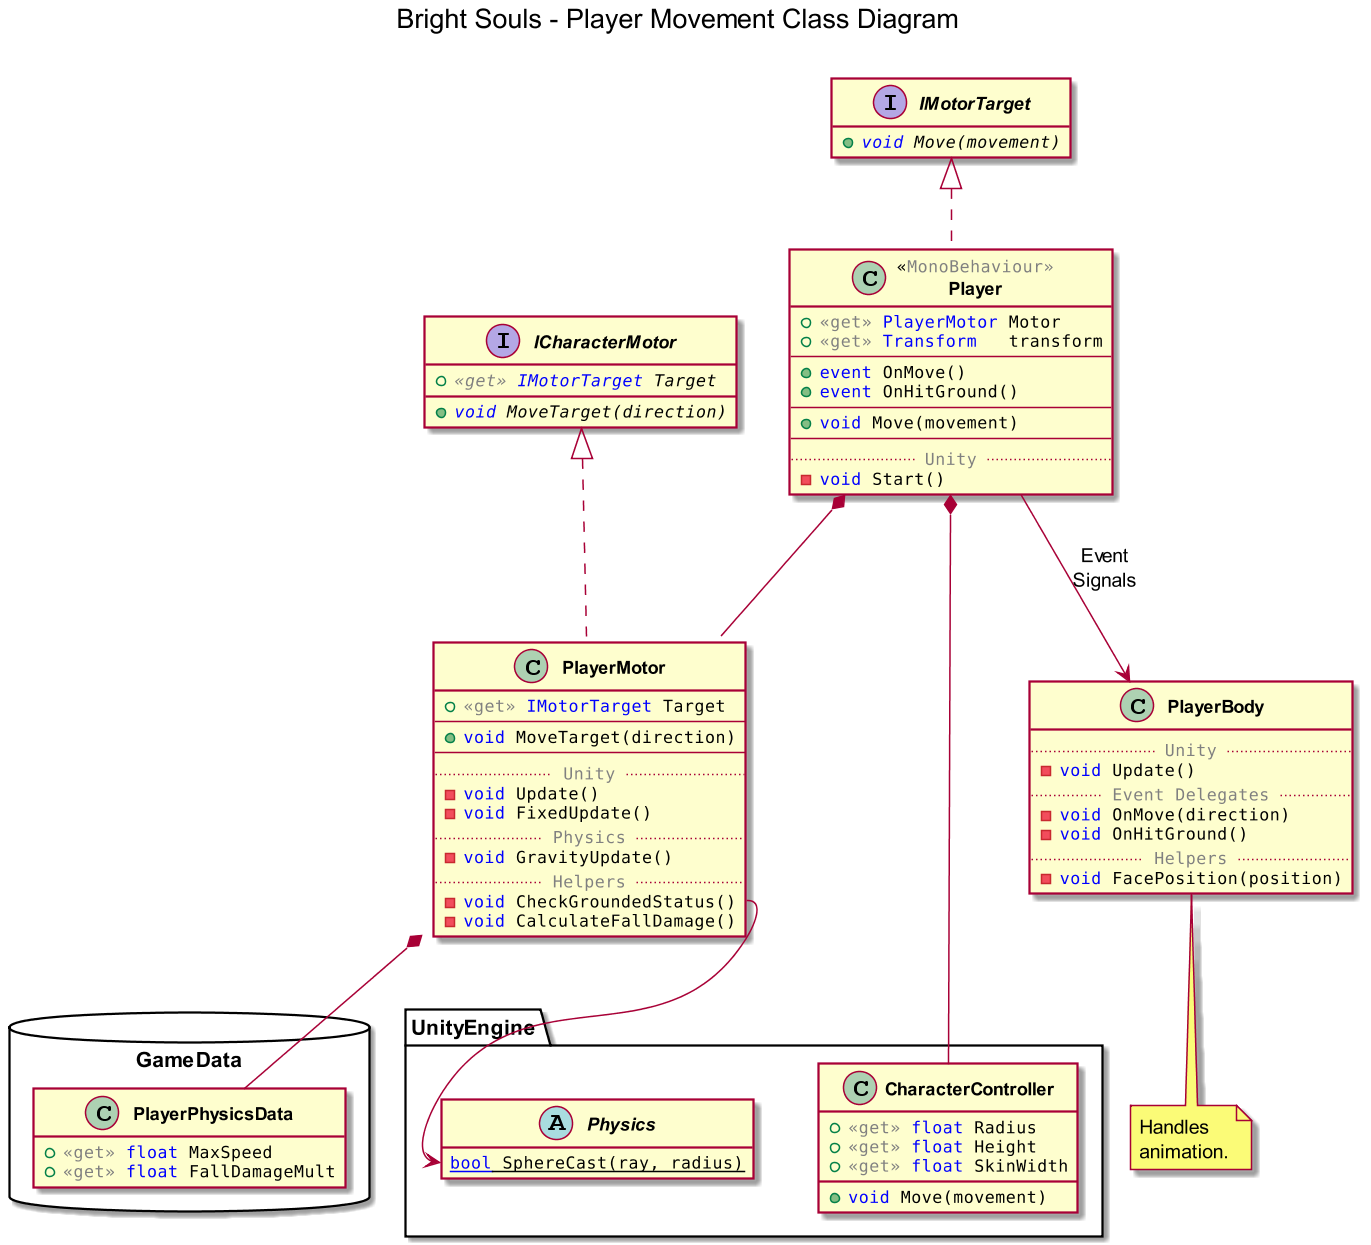
\includegraphics[width=30em]{figures/fig-player-movement-class-diagram.png}
    \end{center}
    \legend{Source: Diagram assembled by authors.}
    \label{fig:movement-class-diagram}
\end{figure}

% ============================================================================
% ============================================================================
% ============================================================================

\subsubsection{Camera System}
\label{sec:lock-on-camera}

% In this implementation, we design and implement two separate camera modes
%   - Orbital Third Person Camera
%       > Commonly used for third person hack n' slash or platforming games
In our implementation, we use our analysis of \emph{Dark Souls} in section \ref{sec:analysis-dark-souls} to design two separate camera modes with complementary functionality that can be used as tools for the player to achieve optimal performance in and out of combat. First we implement an \emph{Orbital Third Person Camera}, which is commonly used in third person \emph{Hack and Slash} and \emph{Platforming} games where the player has to evaluate the properties of the environment they are in and quickly assess dangers that might cause their defeat to devise a plan of action.

%       > Camera positions itself in the perimeter of an ellipsoid that is centered on the player
%       > Input from the player generates movement along the perimeter, causing the camera to orbit around the player
%       > Attempts to frame both the player and the environment by using a position above the player as pivot
An Orbital Third Person Camera positions itself in the perimeter of a three dimensional ellipsoid that is centered on the player, where input from the player generates movement along this perimeter. This type of camera attempts to frame both the player and the environment at the same time, having the player on a central position in the screen and using a position above the player as a rotation pivot. The rotations from player input along with the framing algorithm causes the camera to perform an orbital movement.

%       > In our game, it is the default camera mode, used for traversal around the map
%       > Free control over framing enables player to scout for enemies, avoid pitfalls
In our game, Orbital Third Person Cameras are the default camera mode, and are mainly designed for traversal around the three-dimensional environment. The fact that the player has control over the positioning and framing of the camera enables the player with the possibility to scout the environment for pitfalls and enemies before performing movement. This is the perfect type of camera to be used in out-of-combat situations in third person games, as players can gather information safely and use it to devise a plan-of-action.

%   - Lock-On camera
%       > Mostly used in action third person hack n' slash games that have melee combat, although some RPGs also use it
%       > Camera positions itself behind the player and attempts to frame both the player and a target character
The second type of camera in our implementation is the \emph{Lock-On Camera}, which is mostly used in action third-person \emph{Hack and Slash} games that have melee combat. This type of camera positions itself behind the player character, and attempts to frame both the player and a target -- most commonly an enemy character. Whenever the target character moves, the camera adjusts its position and framing to maintain a fixed relative positioning between the player character and their target.

%       > Camera positioning and framing creates fixed "dimensions of movement" of the player relative to a target,
%         making it easier for a player to avoid attacks from that target and find the optimal spacing to land their
%         own attacks
The relative positioning and framing of a Lock-On Camera creates fixed axes of movement between the player character and their target where if a player moves horizontally, they will move in a circle around the target character. Moving forward and backwards adjusts the distance between the player and their target. The purpose of this mechanism is for the player to have better control of spacing during combat, making it easier for the player to avoid attacks and find the optimal distance to land their own attacks.

%       > Useful for the player to be able to track and attack a single target with ease without missing,
%         instead of having to specify a "direction" for the attack, the player can simply press the attack button
%         and the character will already be facing the enemy and perform the attack in the correct direction
The fact that a Lock-On Camera is always facing a single target character removes the necessity for players to specify a direction for their attacks through input. Instead, players can simply press the attack button when their characters are within attack range. Since the character is constantly facing the enemy, the direction of their attack is guaranteed to be correct. Another positive effect caused by this behavior is that the framing helps the player to focus on the actions being performed by the enemy character, helping to understand when an enemy is attacking and which kind of attack an enemy is performing.

%       > Has issues in environments in constrained spaces, where the enemy is too close to the player or the player
%         is too close to a wall. Framing becomes an issue in this case
However, Lock-On camera implementations face issues when the target character is too close to the player character, or when they are operating in environments with constrained space. When the player character is too close to their target, it is common for Lock-On cameras to not adjust their vertical offset, meaning that the framing direction must be angled downwards and into the ground. This causes the player to have limited geometric information about the surroundings of both characters, making it harder to efficiently navigate the environment during combat. Furthermore, if a player is moving horizontally when close to their target, the perimeter of the circle of movement has a significantly reduced radius, making the camera rotate at high speeds and causing motion sickness\sepfootnote{fn:motion-sickness} in some instances.

When Lock-On cameras operate in constrained space, it is common for the default offset position to be located outside the playable space (e.g. inside walls), and thus a position resolution algorithm is required to guarantee that the camera is always in a valid position. The most common algorithm is the pull-forward approach, where if the camera would be located outside the playable space the target position is recalculated so that the camera is brought closer to the player. While this solution works until a certain point, if the player positions their character too close to a wall it might create a situation where it is impossible for the camera to frame both the player and their target, with either the player character occluding the target or the camera focusing solely on the target by being positioned above the player character. In addition, a similar problem to that of players being to close to targets occurs, where in this case the camera might reposition too quickly due to the resolution algorithm.

Figure \ref{fig:camera-types} shows a comparative diagram of both camera types implemented in this work, where four screen captures are used for the Orbital Third Person Camera to illustrate multiple framing angles that can be achieved from player controlled rotations.

% Figure:  Orbital and Lock-On camera framing/rotation
\begin{figure}[!ht]
    \caption{Comparative screenshots showing the difference between the Orbital and Lock-On camera modes.}
    \vspace{0.5em}
    \begin{center}
        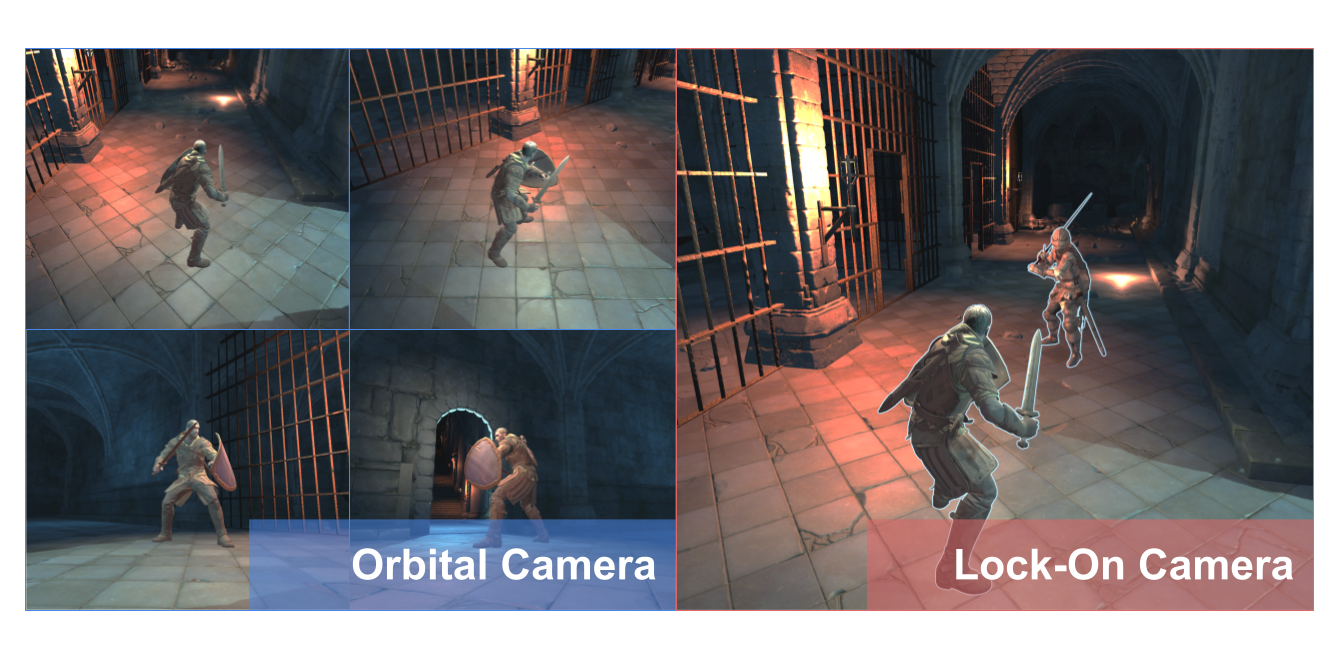
\includegraphics[width=34em]{figures/fig-camera-types.png}
    \end{center}
    \legend{Source: Screen capture of application developed by authors.}
    \label{fig:camera-types}
\end{figure}

% Third Person Orbital Camera implementation
% - Use of Cinemachine
%     * Ready-to use implementation of orbital rotation with parametric spline curve for vertical axis
%     * Smooth transition between virtual cameras which was useful for Orbital Camera and Lock-on modes
Regarding the implementation of the Orbital Camera, we chose to use the \emph{Cinemachine} Unity Package due to its comprehensive API and functionality for multiple types of cameras, including specific algorithms to manipulate Orbital Cameras. Another useful trait is that the APIs provided by Cinemachine enable defining parametric curves for positioning, which increases the expressive power of game designers.

%     * Algorithmic motion that can simulate cinematic behavior with camera shake effect and framing corrections
Cinemachine can also manage, compose and blend multiple cameras, which is useful to perform shot transitions triggered by a signal system that resembles the \emph{Observer} pattern\sepfootnote{fn:observer-pattern}. Cinemachine also includes algorithms for procedural motion generation, which is used to create screen shake effects with high fidelity when the player is attacked by an enemy, or to properly adjust framing when the camera needs to track movement of high velocity targets.

% Prefab GameObject hierarchy with CinemachineBrain at root 
% MainCamera object as a child of the CinemachineBrain
We start by creating a \textsc{Prefab}\sepfootnote{fn:unity-prefabs} hierarchy of \textsc{GameObjects}\sepfootnote{fn:unity-gameobjects} where we include a \textsc{CinemachineBrain} component in the root level, and multiple \textsc{VirtualCameras} as child objects. The \textsc{CinemachineBrain} component is responsible for defining the current active camera, camera transitions and the signals that trigger each transition. The \textsc{CinemachineBrain} brain component requires a reference to a \emph{Main Camera}, a special \textsc{GameObject} with a \textsc{Camera} component responsible for rendering the final output of our camera management system. We add the \emph{MainCamera} object as a child of the root.

% VirtualCamera child objects that contain definitions for transposing and composing strategies
As child GameObjects of the hierarchy root, we include a set of \textsc{VirtualCameras} for each of the camera modes in our implementation. In this case, we simply add a VirtualCamera for the Orbital Camera and another for the Lock-On Camera. VirtualCameras are Cinemachine abstractions that define the physical properties of a camera along with transposing and composing strategies\sepfootnote{fn:transposing-and-composing}. In this case, we use a VirtualCamera with an Orbital transposing strategy and a single LookAt target aiming at a pivot position above the player character. For the Lock-On camera, we use a simple Follow strategy for transposing and a Group Composition strategy to frame both the player character and their target enemy.

% PlayerCameraDirector component, which is responsible for receiving signals from player and translating them into signals for the CinemachineBrain and activating and deactivating PlayerCameraBehaviours
We also add a \textsc{GameObject} containing a \textsc{PlayerCameraDirector} component, which is responsible for receiving signals from the \emph{Player} component and translating them into signals for the \textsc{CinemachineBrain}. The signals are then used to switch and transition between shots. The \textsc{PlayerCameraDirector} is also responsible for enabling and disabling \textsc{PlayerCameraBehaviour} components, which receive player input, manage camera framing targets and initialize camera states.

The \textsc{VirtualCamera} components are tasked with receiving player input and performing the appropriate actions given the input. For instance, the \textsc{OrbitalCamera} receives a two-dimensional vector as input, which is translated into vertical rotation and translation for the Y axis and horizontal for the X axis. In the Lock-On camera, the horizontal axis of the vector input is used to switch Lock-On targets. Figure \ref{fig:camera-class-diagram} shows an overview of the class relationship in our camera system implementation, as well as the signals that are being sent and listened to.

% Figure:  Camera system class diagram
\begin{figure}[!ht]
    \caption{A diagram showing the class relationship of our Camera System implementation, along with the signals being sent and processed.}
    \vspace{0.5em}
    \begin{center}
        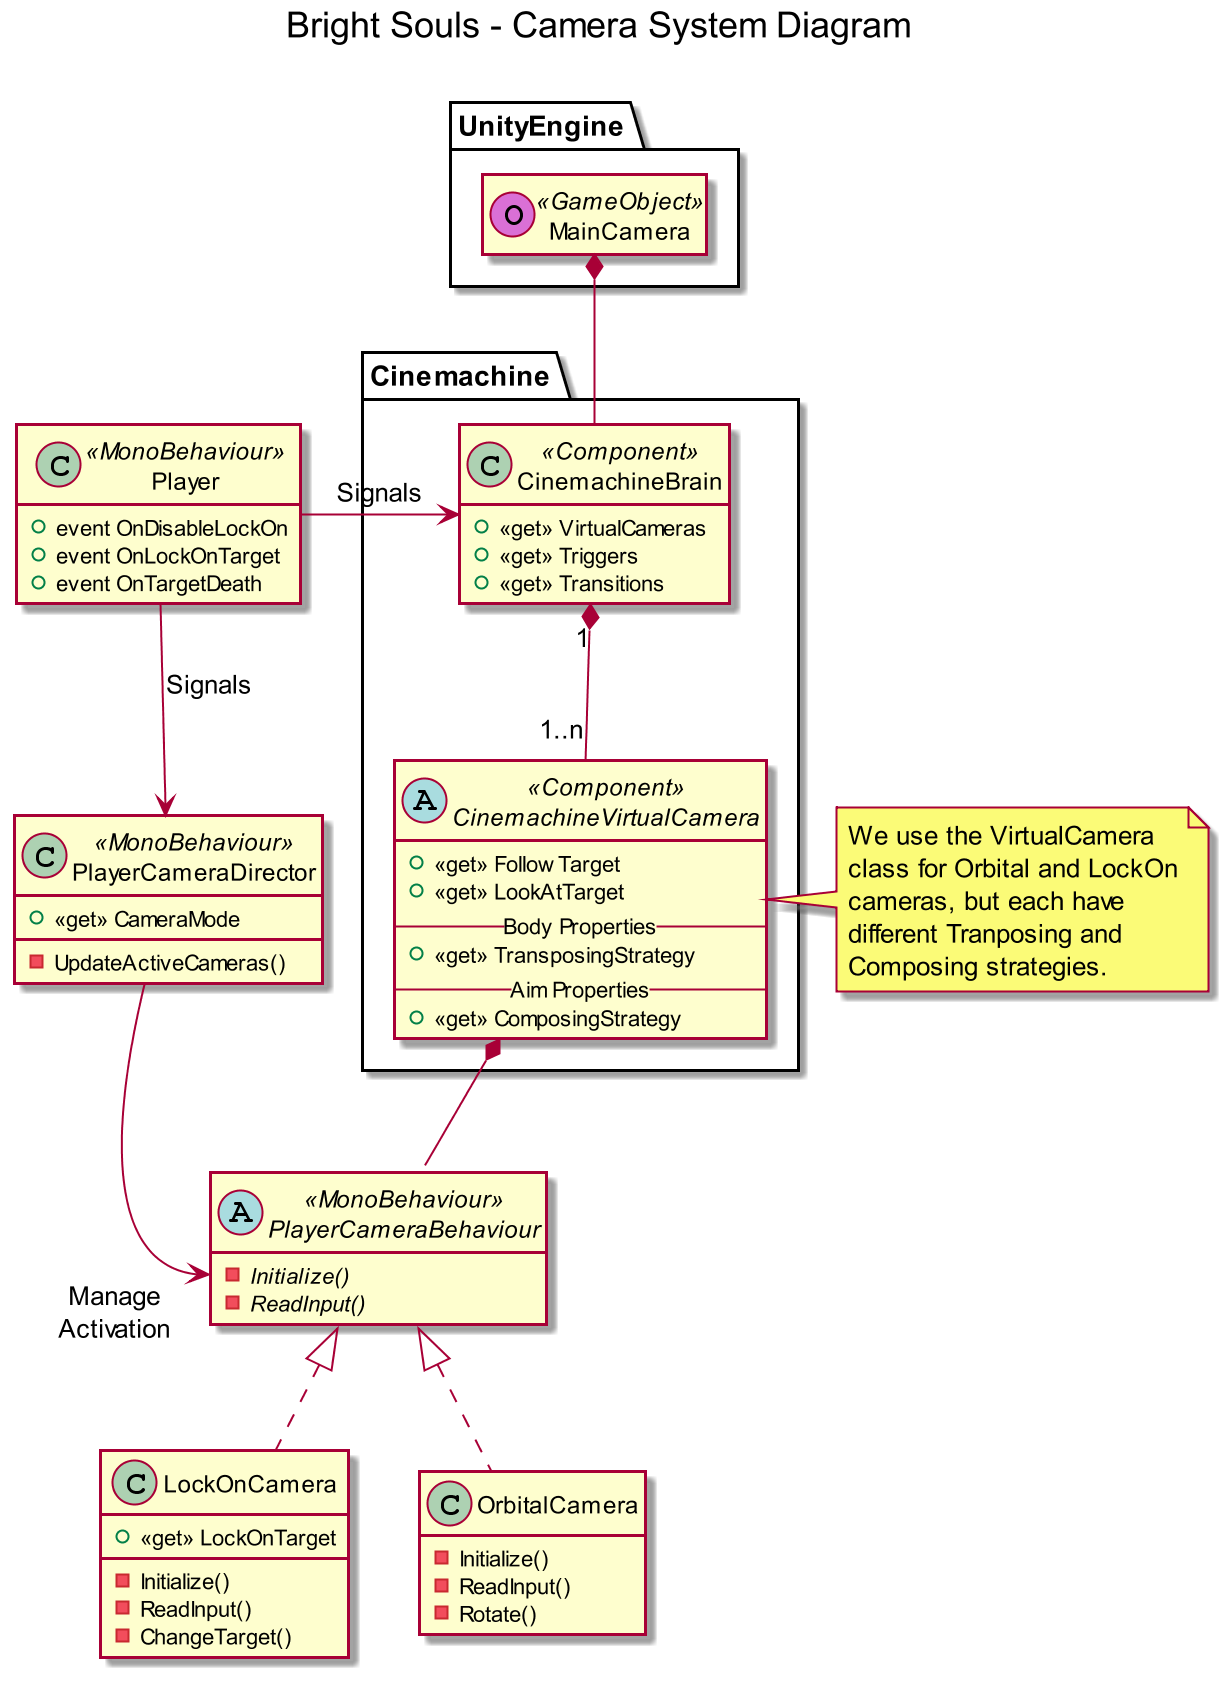
\includegraphics[width=24em]{figures/fig-camera-system-class-diagram.png}
    \end{center}
    \legend{Source: Diagram assembled by the authors.}
    \label{fig:camera-class-diagram}
\end{figure}

%     * Simplified collision geometry enables using a pull-forward collision resolution
For position resolution, we created a simplified and invisible collision map to define the constraints of where a camera can be positioned in a game level. This is done to both improve the performance of raycasts and to avoid jittery movement when using pull-forward collision resolution on thin objects. This collision map is limited to interact with camera algorithms, and does not affect player movement or any other physics entities in any way.

% Lock-On camera and targeting system
% - Possible Lock-on targets must be located in an intersection of the camera viewport with a collision sphere centered at player character
% - Lock-On target prioritization is higher for targets that are closer to the player and to the center of the screen
To detect Lock-On eligible targets, we use a spheric collider in a radius around the player collider and intersect any detected entities with those present in the viewport, to constrain selection to entities being visualized. Eligible targets are collected into a list ordered by distance to the player character, which is updated every second. This is done because targets that are closer to the player are considered a higher threat, as they are more likely to hit the player when attacking.

% - Use of horizontal input axis from Orbital Camera to switch between targets
Horizontal input from the player is used to switch between targets, where moving the input axis to the left switch to the closest target at the left of the current Locked-On target, using coordinates relative to viewport space. Therefore, the position of the next target is selected using a comparison of the position of the entity in the X-axis when converting their coordinates to a viewport space.

\subsubsection{Attributes System}

% Attributes system
Attributes are our abstraction for runtime data that represents the current state of a gameplay entity, such as the Player Character, an Enemy Character or even an interactable object in a level such as a door. Attributes can be initialized, serialized and monitored by external components and are used by a multitude of gameplay related systems. In our implementation, attributes are mostly used to represent combat related variables such as Health, Stamina and Poise, and thus are affected by events triggered by the combat system, such as Stamina being used when the player attempts to attack an enemy, or the Health lost when an enemy succesfully hits the player.

% Based on Generics: Attributes can be generated for any primitive type, such as int, float, double, string.
%   - Serialized into binary gameplay data files for game designers to define the default and maximum values for character health, stamina and poise
%   - Initialized by persistent data managers to maintain player status when transitioning between levels
Attributes are based on \textsc{C\#} \emph{Generics}, and can be generated for any value type such as integers, floating point variables, strings and enumerations. This limitation is imposed in our architecture so that attributes can be easily serialized into binary data files that can be used to define the default and maximum values for each attribute holder. This constraint also facilitates Attribute initialization, which is useful to support persistent data such as maintaining attributes between levels  or loading the state of an entity from a file in a savegame system. 

%   - Monitored by UI systems to display relevant data about the status of the player, for instance a Health Bar that display the current health of the player and shows health lost when getting attacked.
All Attribute types implement the \textsc{IAttribute} interface, which exposes acessors for data manipulation and events for value changes. This facilitates the use of attributes by separate, independent systems in our architecture. For instance, Attributes are monitored by UI (User Interface) systems to display relevant data about gameplay entities, such as the status of the player. Health bars show the current player health and also provide a good estimation of health lost when getting attacked by an enemy using a secondary, trailing health bar.

The advantage of creating of an event monitoring system between Attributes external systems is that upon initial conception of the architecture, we do not exactly know how many components will require communication with each gameplay entity. For instance, when implementing the UI for the player character we can initially propose a single health bar that would simply read the value of runtime variables from the \textsc{Player} class, but if we iteratively add new elements such as floating text, combat messages and visual effects, each of these systems should have direct access to the components that hold data regarding player state, which enforces component coupling in our architecture. With an event system, we can simply subscribe to signals being sent by attributes, constraining the exposed data and methods and facilitating component decoupling.

% - AttributesContainers
%     * Containerization of attributes to allow for entities with different attribute configurations without defining static types
%     * Possibility to dynamically assign attributes during the course of a session, which can be useful for a telemetry system
% - Definition of interfaces that expose attributes to any of the classes that might require it
Attribute owners will often contain different sets of attributes to satisfy the requirements of the systems they interact with. As such, characters that can partake into combat encounters will present different attributes in relation to interactable objects such as doors. To provide a standardized interface for the access of attributes over different entity types, we containerize attributes into \emph{Attribute Containers}, which provide a public interface for dynamic access and manipulation of statically typed attributes contained within an entity. Figure \ref{fig:attributes-diagram} shows an overview of the class relationships in the Attributes System, along with examples of how attributes signalize changes to external components such as UI Elements.

% - Figure: Attributes system class diagram
\begin{figure}[!ht]
    \caption{Class diagram for the Attributes System, showing examples of signals being used by UI Elements.}
    \vspace{0.5em}
    \begin{center}
        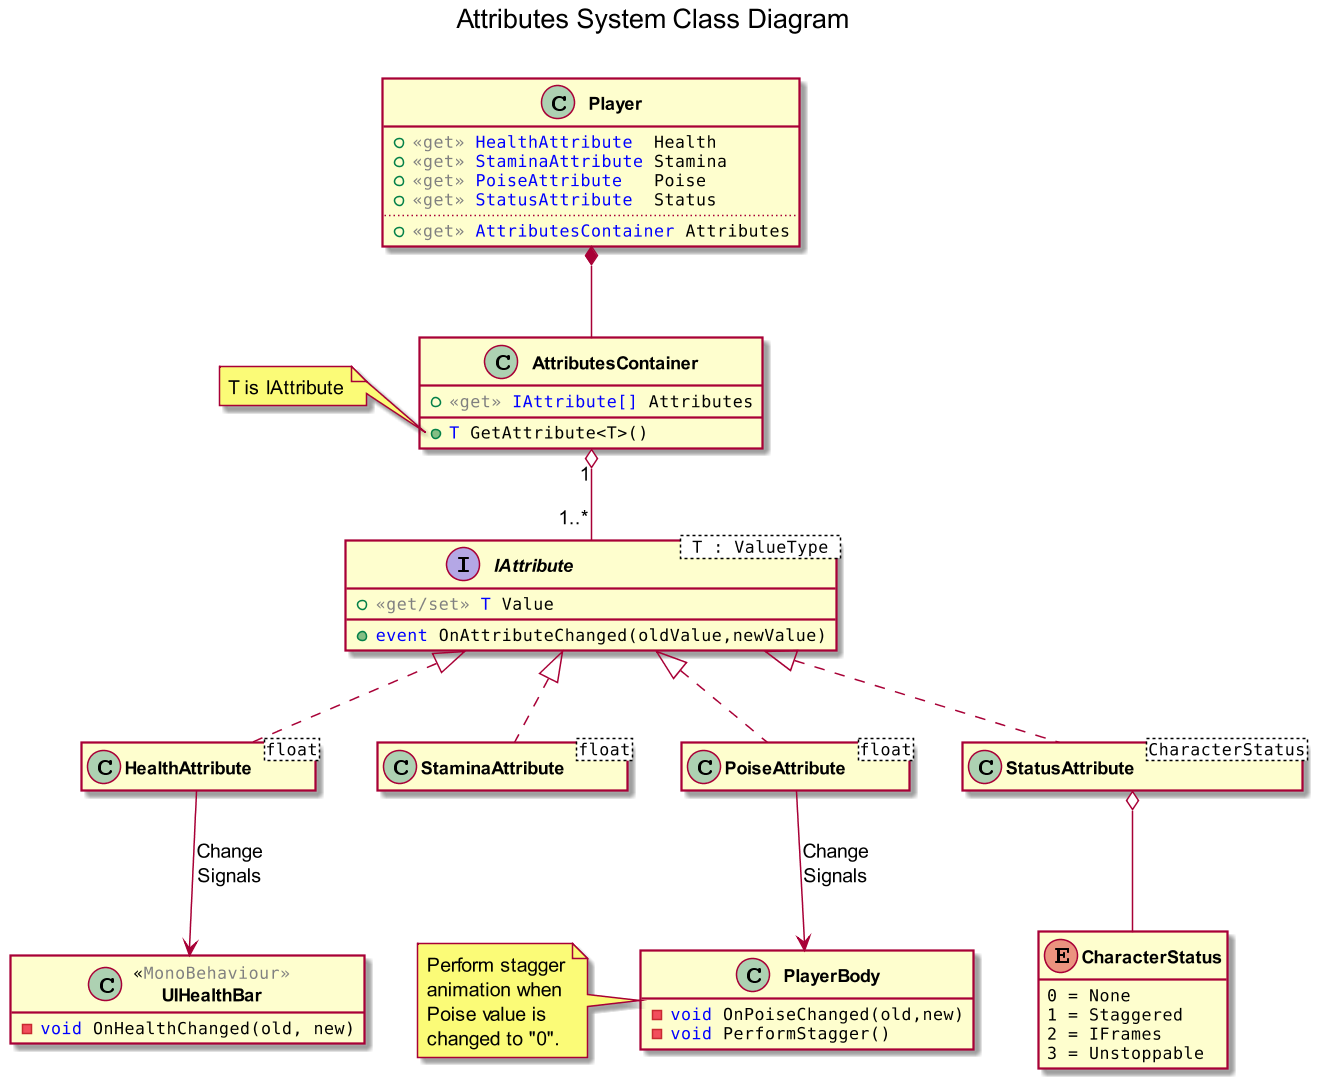
\includegraphics[width=34em]{figures/fig-attributes-diagram.png}
    \end{center}
    \legend{Source: Diagram assembled by the authors.}
    \label{fig:attributes-diagram}
\end{figure}

\subsubsection{Combat System}

% Combat System involves:
% - Managing attacking and combo animation and logical states for the player
% - Being able to detect when the weapon of the attacker collides with a target
% - Being able to detect when the target was able to block or dodge an attack
% - Applying combat effects when the target is hit
To implement combat-related mechanics for a \emph{Souls-like} game, we need a set of functionality components that are able to:
\begin{itemize}
    \item{Manage attack animations and logical states for the player character;}
    \item{Detect when the weapon of the attacker overlaps with the body of a target to validate a \emph{Succesful Hit};}
    \item{Apply \emph{Combat Effects} when a target is hit by an attack, such as a \emph{Health Damage} effect;}
    \item{Verify if attacks are blocked or dodged, and apply modifiers or even nullify Combat Effects;}
    \item{Modify character state according to the effects that are applied.}
\end{itemize}
By combining the functionality aforementioned with AI agents that also make use of the same components, we can create a simple but credible Combat System that provides appropriate feedback to player actions and decisions. In figure \ref{fig:combat-system-overview}, we provide an overview of the subsystems and classes regarding to our implementation of a Combat System.

% Figure: Combat System Overview Diagram

% Attacking and combo system
%  - Continuously check for Attack input
We begin by listening to input from the player to determine when an \emph{Attack Command} should be issued. If the button mapped to the \emph{Attack Command} is pressed, we proceed to verify the current state of the player character to determine if an attack can be performed. The current state of the player is defined by a composition of boolean variables that reflect by the Animation being played on their character model.

% - Player/character is unable to perform attack if on Animation Lock
% - Attacks cost Stamina
If the character model is in the \emph{Dead}, \emph{Staggered}, \emph{AttackEnding}, \emph{On-Air}, \emph{Landing}, \emph{Dodging} or \emph{Blocking} animation states, the player is unable to perform an attack. This is commonly referred as \emph{Animation Locking} in games, and is an important aspect to potentially punish the player when taking strategically negative decisions. Attack Commands also have a resource cost for the player, where each attack depletes an amount of \emph{Stamina}. If the player Stamina resource has a value of zero, the player is unable to perform an attack. If the player has any Stamina value above zero, they are able to perform the attack.

%  - When sending attack command, enter a "combo" state and "Attack animation state machine"
%  - "OnCombo" state:
%    * Preemptively read player input before current attack animation ends. If player successfully sent attack input, continue the combo.
%    * If no attack input command is read within animation time frame, escape the Attack animation state machine
After an Attack Command is successfully validated, player state is set to \emph{Attacking} and the player enters an \emph{Attack State Machine} where Attack Commands are preemptively verified during attack animations. If an Attack Command is successfully executed before an attack animation ends an \emph{Attack Chain} is toggled, meaning that another attack animation is queued and transitioned to when the current attack animation ends. This behavior is commonly referred to as a \emph{Combo} in video games.

This replicates how attacking works in Dark Souls, where the player can continuously enqueue attack commands until their \emph{Stamina} resource is depleted. If no Attack Command is successfully executed within the time frame of an attack animation, the player exits the \emph{Attack State Machine} and is locked to a short \emph{AttackEnding} animation state, where the player character model transitions from attacking to an idle state.

% Figure: Attack and combos Class Diagram

%   > Hit detection toggled when receiving an event signal from the Attack animation
During Attack animations, the Animation System broadcasts event signals that toggle the activation and deactivation of the \emph{Hit Detection System}, which has the purpose of determining whether an attack successfully hit an enemy. At a certain point during the attack animation, we broadcast the \emph{AttackCollisionStartEvent} which signalizes that attack collisions must be checked on each frame until an \emph{AttackCollisionEndEvent} is signalized. The \emph{AttackCollisionEndEvent} is required to be signalized after the \emph{AttackCollisionStartEvent} and before the attack animation ends so that attacks appropriately reflect what the attacking character performs. Generally, the point in time at which \emph{AttackCollisionStartEvent} and \emph{AttackCollisionEndEvent} are triggered should occur in the small time frame where the character swings the weapon in the direction of their target.

%     * Hit detection must not occur twice between the same target and same attack
%     * Specific collision layer to detect hitbox collision
To implement hit detection, we perform collider overlap checks in fixed time intervals of 16 milliseconds. These collision checks occur in a special collision layer called HitDetection, where every Collider is either the weapon of an attacker or the body of a target. This is an optimization requirement to meet the required time constraint in most computing systems. If a system is unable to meet the time constraint, there is a small chance that an attack might not be detected, where the attacker weapon "passes-by" the body of the attacker without triggering collision detection.

We estimate that attack collision detection occurs for approximately 20 frames from the point where it is first activated. Thus, if a computer system is able perform at least 4 updates per second, attack collision is guaranteed to be correctly detected. It is important to note that updates to the collision detection system are independent to the rendering performed by the graphics pipeline, and as a consequence are unaffected by most forms of temporary stutters in the application.

We also require safety measures to ensure that attack collision detection does not trigger a Hit event twice given the same Attack and Target entities. Therefore, for each attack performed by an attacking entity that is successfully registered as a Hit, we store a reference to an \emph{AttackCollision} instance in the \emph{Hitbox} component of the target entity. The Hitbox component then listens for the \emph{AttackCollisionEndEvent}, where the reference can be deleted since at this point the same \emph{AttackCollision} instance is not performing any collision checks.

% - Hit detection:
%   > Colliders:
%     * Hitbox overlap detection for attacker weapons and target character
%     * Attack Colliders are bounding boxes in weapons
%     * Character colliders are simplified bounding boxes that enclose torso, head and partially legs
For each occurrence of an attack collision, two colliders are obligatorily involved: one for the weapon of the attacker, and one for the body of the target. The colliders are instanced as \emph{bounding boxes}\sepfootnote{fn:bounding-boxes} that fully or partially enclose the 3D models of their relative entity. In order to perform collision checks with a reasonably optimized numbers of collision checks, we simplify bounding boxes of character models to only enclose the torso, head and a central position of the legs of a target. Using this method, we can minimize the amount of collision checks per frame, while also having appropriate precision for our implementation purposes.

%     * Consider character faction to recognize which combat characters can be hurt by an attack
After the collision detection step is performed, we must ensure that the attacking character is hitting a target that is not part of their own \emph{Combat Group} before validating an attack as a \emph{Successful Hit}. To do this we create the \emph{Faction Attribute}, which determines that each character belongs to a combat group that is unable to perform attacks to other members of the same group. This is done so that groups of characters such as enemies of the player do not damage themselves when attempting to hit a target while being too close to each other. The values that the faction attribute can be assigned are described in table \ref{tab:table-faction-groups}.

\begin{table}
    \begin{center}
      \caption{A description of the values that can be assigned to the \emph{Faction Attribute} of targets that are part of the Combat System in our implementation.}
      \label{tab:table-faction-groups}
      \rowcolors{2}{}{gray!25} % Alternate row colors
      \begin{tabular}{ >{\small}w{l}{3em} >{\small}w{c}{3em} m{25em} } % alignments and column size
        \addlinespace
        \toprule
        % Headings
        \bf Name    & \bf Id   & \bf Description                                              \\
        \midrule
        % 3D Models
        Player       &       0 & Player character. The player is a single entity and the sole 
                                 participant of this faction group.                           \\

        Enemy        &       1 & AI Agents that represent Enemies, which are hostile to the 
                                 player character.                                            \\

        NPC          &       2 & Non-Playable Characters. AI Agents which are not hostile to 
                                 the player character, but are hittable by and potentially 
                                 hostile to Enemies. An example of a Non-Playable Character 
                                 would be a companion which follows the player character and 
                                 aids them in combat encounters, being hostile to characters 
                                 belonging to the Enemy faction.                              \\

        Interactable &       3 & Static objects that can be attacked by the Player, Enemies or 
                                 Non-Player Characters and provide some type of feedback when 
                                 attacked. An example of an interactable entity would be a 
                                 barrel that can be attacked and destroyed.                   \\
        \bottomrule
      \end{tabular}
    \end{center}
  \end{table}

% Figure: Hit detection class diagram

% - Attack damage and other effects are abstracted into Combat effects
%     * Manipulate character attributes, statuses and physics
%     * Instant combat effects are completely applied in the same frame as hit detection occurred
%     * Over-time combat effects with fixed interval ticks
% - Combos: 
%     * Detecting and queuing input commands during attacking animations to allow for chained attacks
%     * Alternating between attack animations to create the impression of a seamless combo that is only limited by the stamina resource

% - Combat Effect Modifiers
%     * Block detection occurs when target is hit, is in "blocking" state and vector dot product between attack and target directions is < 0
%     * Dodge detection also occurs when target is hit. If hit detection occurs during target invincibility frames, a "dodge" is registered, and target receives no combat effects

% Player has a default Stamina regeneration effect
The player character has a a default Stamina regeneration \emph{Combat Effect} that is temporarily blocked or modified by combat-related actions. After a certain amount of time without issuing combat-related commands such as Attacking and Dodging, Stamina regeneration is re-enabled. Entering the Blocking state applies a modifier to the Default stamina regeneration, where the Stamina value recovered is halved. 

% Figure: Combat Effect class diagram

\subsubsection{Animation System}

% Animation system
% - Difference in body movement when in Orbital vs Lock-On Cameras
% - React to attribute changes, motor velocity and physics updates

% - Figure: Player Animation State Machine

% - Statuses such as staggered, dead will override other animations
% - Blending between animations states when performing directional actions
% - Transitioning between combo states
% - Animation events for hit detection when attacking

% - Figure: Animation System class diagram showing component relations and events

\subsection{Artificial Intelligence}

% Enemies in Dark Souls present basic, somewhat predictable behavior

% We chose to implement AI agents using State Machines given the target simplicity of Enemy Behavior

% Figure: State Machine system architecture


% Figure: Melee enemy AI State Machine
\begin{figure}[!ht]
    \caption{An example of the State Machine that represents a Melee Enemy AI Agent. Each state holds its own behavior.}
    \begin{center}
        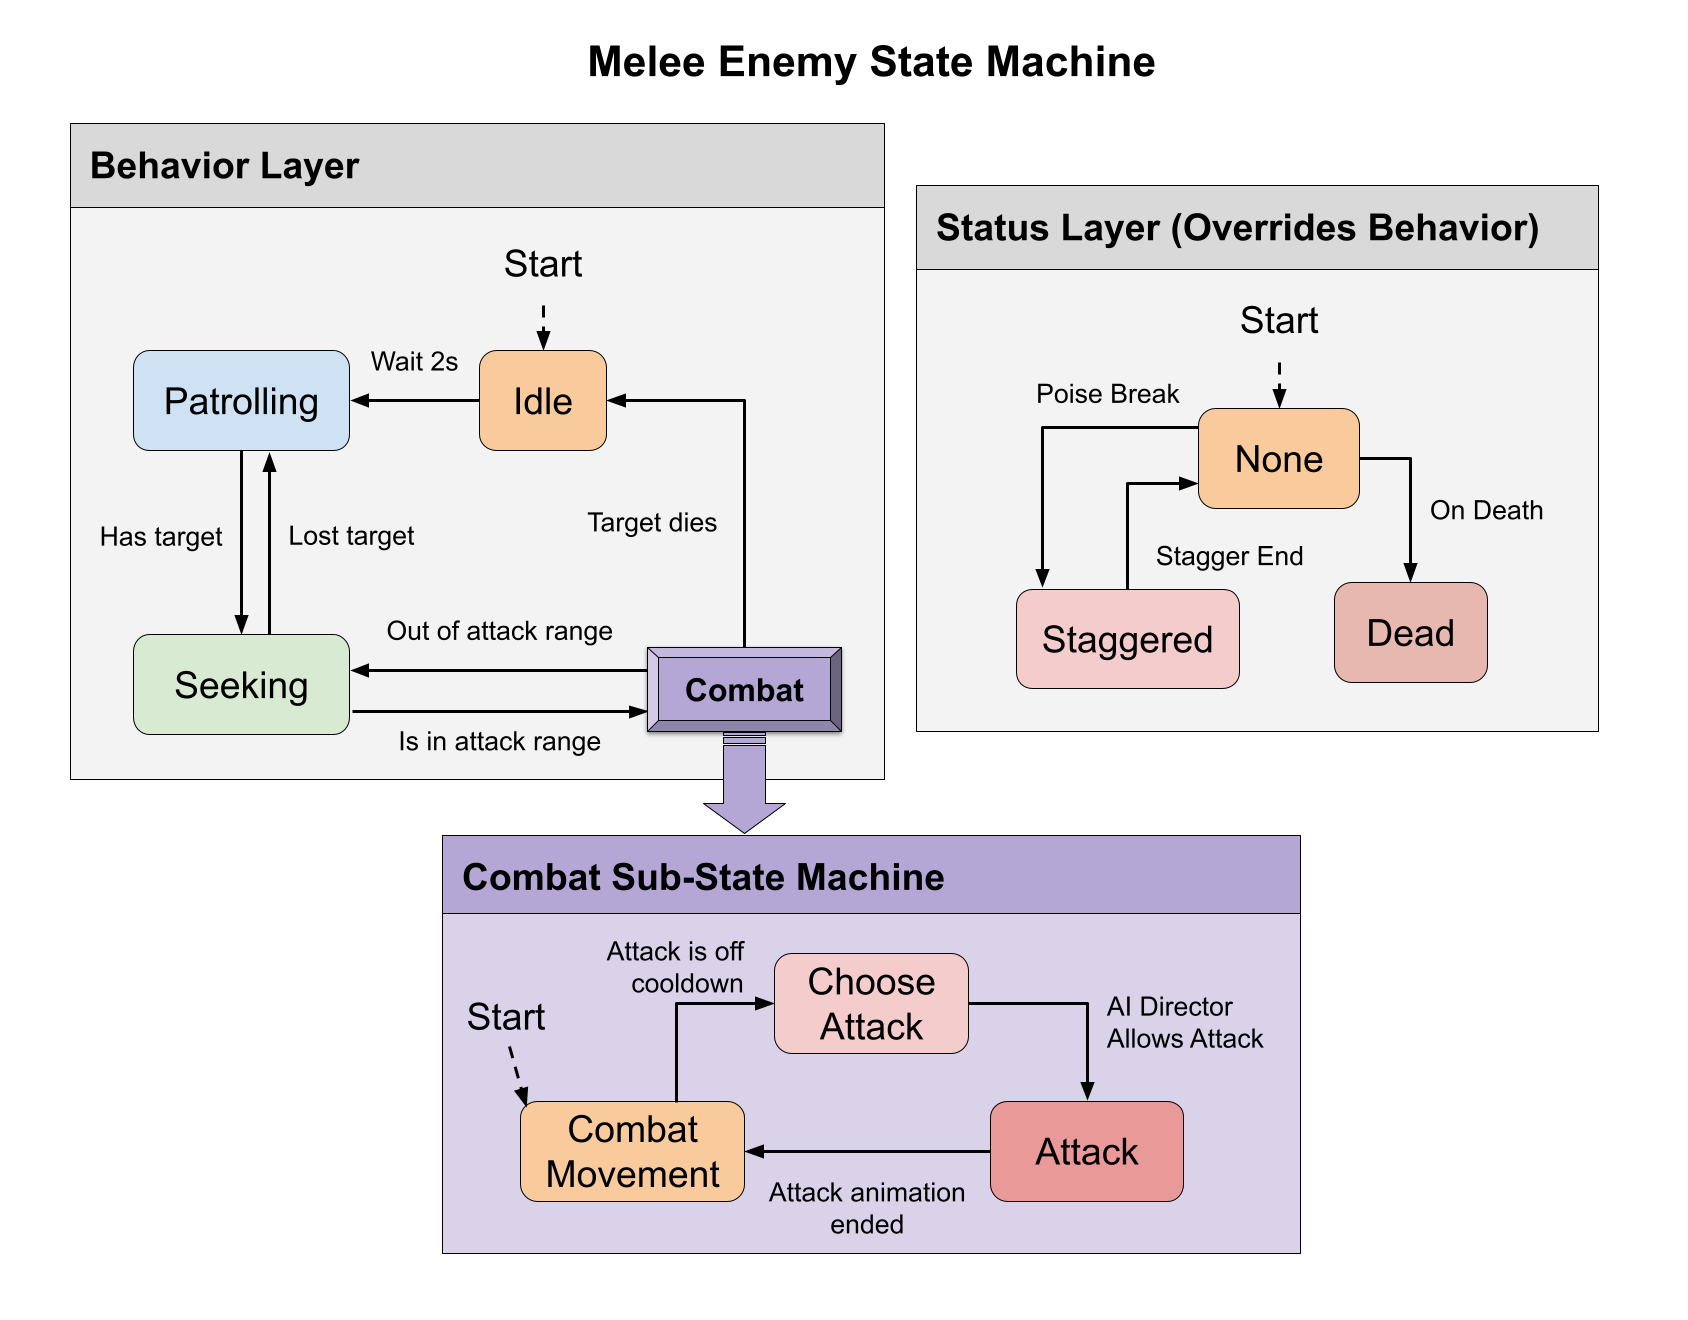
\includegraphics[width=34em]{figures/fig-melee-ai-state-machine.png}
    \end{center}
    \legend{Source: Diagram assembled by authors.}
    \label{fig:fig-ai-state-machine}
\end{figure}

\subsection{Telemetry and Performance Tracking}

\subsection{Dynamic Adjustments}

\section{Experimentation Model}

\subsection{Methodology}

\subsection{Results and Analysis}

\section{Conclusions}

% limitations

% comparison with previous work